\section{Introduction}
Graphs are widely used to model relationships and interactions 
in data from multiple domains, such as network analysis, bioinformatics, and chemistry. 
Many learning tasks are defined at the graph level. 
However, graphs exhibit irregular structures with variable sizes and features, 
which pose challenges for traditional machine learning algorithms.

Graph embedding methods address these limitations by mapping entire graphs 
into fixed-size vector representations, enabling standard machine learning techniques 
to be applied efficiently to downstream tasks. 
Early approaches based on handcrafted features or graph kernels 
suffer from high computational complexity or limited expressiveness~\cite{shervashidze2011wl,vishwanathan2010graphkernels}. 
More recent methods automatically learn graph representations and can be broadly categorized into 
unsupervised~\cite{narayanangraph2vec,tsitsulin2018netlsd} and supervised techniques
~\cite{xu2019gin}.

\begin{figure}
    \centering
    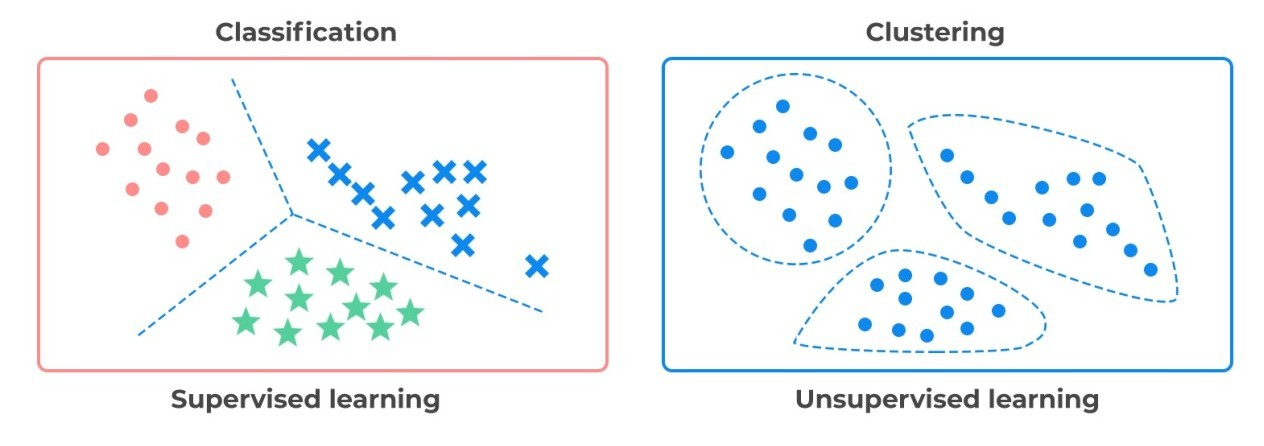
\includegraphics[width=\linewidth]{figures/svsu1.jpeg}
    \caption{Comparison between unsupervised (a) and supervised learning (b).}  
    \label{fig:SupervsUn}
\end{figure}

Figure~\ref{fig:SupervsUn} illustrates the conceptual difference between unsupervised and supervised graph embedding methods. 
In the supervised setting graph representations are learned solely from the graph structure and 
feature similarity without access to label information. 
As a result, the embedding space organizes graphs into clusters which may correspond to 
latent communities but are not explicitly aligned with semantic classes. 
In contrast, supervised graph embedding methods leverage labeled data during training to 
shape the embedding space. 
Graphs belonging to the same class are encouraged to be close as we can see from the figure, 
while graphs from different classes are pushed apart leading to embeddings that are explicitly discriminative and 
separable by a decision boundary. 
This distinction highlights how supervision guides representation learning toward task specific objectives, 
such as graph classification, whereas unsupervised embeddings primarily capture the underlying geometry 
and connectivity of the graph.


Despite their success, supervised methods require labeled data 
and typically incur higher computational costs due to iterative training, 
whereas unsupervised methods do not require labels and are generally more efficient. 
However, systematic comparisons between these two paradigms remain limited, especially 
on small benchmark datasets where robustness and efficiency are critical~\cite{errica2019fairgnn,dwivedi2020benchmarking}.

In this work, we focus on the EMB1 setting and our purpose is to compare unsupervised and supervised 
graph embedding methods on small benchmark datasets from TUDataset. 
We evaluate Graph2Vec, NetLSD and GIN under a unified experimental 
framework, considering not only classification performance 
but also clustering quality, computational cost and stability to structural perturbations.
To guide our empirical evaluation, we address the following questions:
\begin{itemize}
    \item \textbf{RQ1:} How do unsupervised graph embedding methods compare to supervised GNN-based approaches in terms of classification performance on small benchmark datasets?
    \item \textbf{RQ2:} How well do different graph embeddings capture graph similarity, as reflected by clustering quality?
    \item \textbf{RQ3:} What are the computational efficiency trade-offs between unsupervised and supervised methods?
    \item \textbf{RQ4:} How robust are graph embeddings to structural perturbations of the input graphs?
\end{itemize}

So our contributions are summarized as follows:
\begin{itemize}
    \item A unified and fair experimental framework for comparing supervised and unsupervised graph embedding methods on small datasets
    \item An analysis of performance–efficiency trade offs, and
    \item An evaluation of embedding robustness under structural perturbations. 
\end{itemize}


